\documentclass[11pt]{ctexart}
% \documentclass{article}
\textheight 23.5cm \textwidth 15.8cm
%\leftskip -1cm
\topmargin -1.5cm \oddsidemargin 0.3cm \evensidemargin -0.3cm

\usepackage{verbatim}
\usepackage{fancyhdr}
\usepackage{graphicx}
\usepackage{amssymb}
\usepackage{amsmath}
\usepackage{booktabs}
\usepackage{subcaption}
\usepackage{listings}
\usepackage{color}
\usepackage{geometry}


\definecolor{mygreen}{rgb}{0,0.6,0}
\definecolor{mygray}{rgb}{0.5,0.5,0.5}
\definecolor{mymauve}{rgb}{0.58,0,0.82}

\lstset{
  language=Matlab,                % 设定语言为MATLAB
  frame=single,                   % 外围框架
  basicstyle=\footnotesize\ttfamily,   % 基本代码风格
  keywordstyle=\color{blue},      % 关键词风格
  commentstyle=\color{mygreen},   % 注释风格
  stringstyle=\color{mymauve},    % 字符串风格
  numbers=left,                   % 行号位置
  numberstyle=\tiny\color{mygray}, % 行号风格
  stepnumber=1,                   % 行号步长
  numbersep=5pt,                  % 行号与代码间隔
  backgroundcolor=\color{white},  % 代码背景色
  showspaces=false,               % 不显示空格
  showstringspaces=false,         % 不显示字符串中的空格
  showtabs=false,                 % 不显示制表符
  tabsize=4,                      % 制表符宽度
  captionpos=b,                   % 标题位置
  breaklines=true,                % 自动换行
  breakatwhitespace=false,        % 仅在空格处换行
  escapeinside={\%*}{*)},         % 可以添加LaTeX内容
}


\ctexset {
     section/format    += \sffamily\raggedright,
     subsection/format += \fbox,
}


\title{FEM Code Report 1}
\author{SA24229016 王润泽}

\begin{document}
\maketitle

\section{Introduction}
	编写程序求解以下两点边值问题(1):
	\begin{equation}
		\begin{aligned}
			-u'' &= f, \quad 0 < x < 1, \\
			u(0) &= u(1) = 0.
		\end{aligned}
	\end{equation}
	其中取 $ f(x) = -(2\cos{x}-(x-1)\sin{x}) $,已知其解析解为 $ u(x) = (x-1)\sin{x} $。
\section{Method}

	给定双线性形式 $a(u,v)$ 和内积 $(f, g)$,定义如下:
	\begin{equation*}
		\begin{aligned}
			a(u,v) &= \int_0^1 u' v' \, dx, \\
			(f, g) &= \int_0^1 f \cdot g \, dx.
		\end{aligned}
	\end{equation*}

	由此,问题 (1) 转变为变分问题(2):

	寻找 $u \in \mathcal{V} = \{v \in C[0,1], v(0) = v(1) = 0\}$,使得对所有 $v \in \mathcal{V} $,均有:
	\begin{equation}
		a(u,v) = (f,v).
	\end{equation}

	实验中采用等距网格划分,节点数为 $N+2$,在每个节点处的函数值记为 $u_i$,且已知 $ u_0 = 0, u_{N+1} = 0 $  ,网格步长为 $h = 1/N$。选取基函数 $\varphi_i$,并通过这些基函数所张成的有限维线性空间 $ V_h=\text{span}\{\varphi_i\} $ 进行求解。此时得到原问题的离散形式解为:$ u_h = \sum_{i=1}^{N} u_i \varphi_i $,其中 $u_i$ 为待求解的系数, 而 $ v_h = \sum_{i=1}^{N} v_i \varphi_i $。 

	此时变分问题的离散形式为问题(3):	
	\begin{equation}
		\begin{aligned}
			a(u_h, v_h) &= \sum_{i=1}^{N} \sum_{j=1}^{N} u_i a(\varphi_i, \varphi_j) v_j \\
			(f, v_h) &= \sum_{i=1}^{N} f_i v_i
		\end{aligned}
		\label{eq:discrete}
	\end{equation}
	
	实验中基函数定义如下:
	\begin{equation}
		\varphi_i(x) = 
		\begin{cases} 
		\frac{x - x_{i-1}}{x_i - x_{i-1}}, & x \in [x_{i-1}, x_i), \\
		\frac{x_{i+1} - x}{x_{i+1} - x_i}, & x \in [x_i, x_{i+1}], \\
		0, & \text{otherwise}.
		\end{cases}
		\label{eq:basis}
	\end{equation}
	
	得到公式 \eqref{eq:discrete}中刚度矩阵各项:
	\begin{equation} 
		a(\varphi_i, \varphi_j)=\left\{
		\begin{aligned}
			&-\frac{1}{h}, & |i-j| = 1\\
			&\frac{2}{h}, &i = j\\
			&0,  &\text{otherwise}
		\end{aligned}
		\right.
	\end{equation}
	
	因此,刚度矩阵为:
	\begin{equation}
		A = \frac{1}{h}\begin{bmatrix}
			2 & -1 & 0 & \cdots & 0 \\
			-1 & 2 & -1 & \cdots & 0 \\
			0 & -1 & 2 & \cdots & 0 \\
			\vdots & \vdots & \vdots & \ddots & \vdots \\
			0 & 0 & 0 & \cdots & 2
		\end{bmatrix}
	\end{equation}

	同理,根据公式 \eqref{eq:basis},得到对各个基函数与 $f$ 的内积,即荷载向量各项为:
	\begin{equation}
		f_i = (f, \varphi_i) = \int_0^1 f \varphi_i \, dx = 4(hj-1)\sin^2(h/2)sin(hj)/h-2\sin(h)\cos(hj)
	\end{equation}

	以上,得到变分问题的离散形式为,对任意的 $ V=(v_1,v_2,\cdots,v_{N})^T $,有: 
	\begin{equation}
		V^TAU = V^TF
	\end{equation}

	进一步,只要求解出 $ AU = F $ 即可得到 $ U $,即为问题 (1) 的数值解,其中:
	\begin{equation}
		\begin{aligned}
			U &= (u_1, u_2, \cdots, u_{N})^T, \\
			F &= (f_1, f_2, \cdots, f_{N})^T.
		\end{aligned}
	\end{equation} 

\section{Results}

\subsection{数值拟合效果}
通过调整 $N=\{10,20,40,80\}$ 的值,得到不同的数值解,与解析解进行比较,如图 \ref{fig:fit} 所示。

\begin{figure}[h]
    \centering
    \begin{subfigure}{0.4\textwidth}
        \centering
        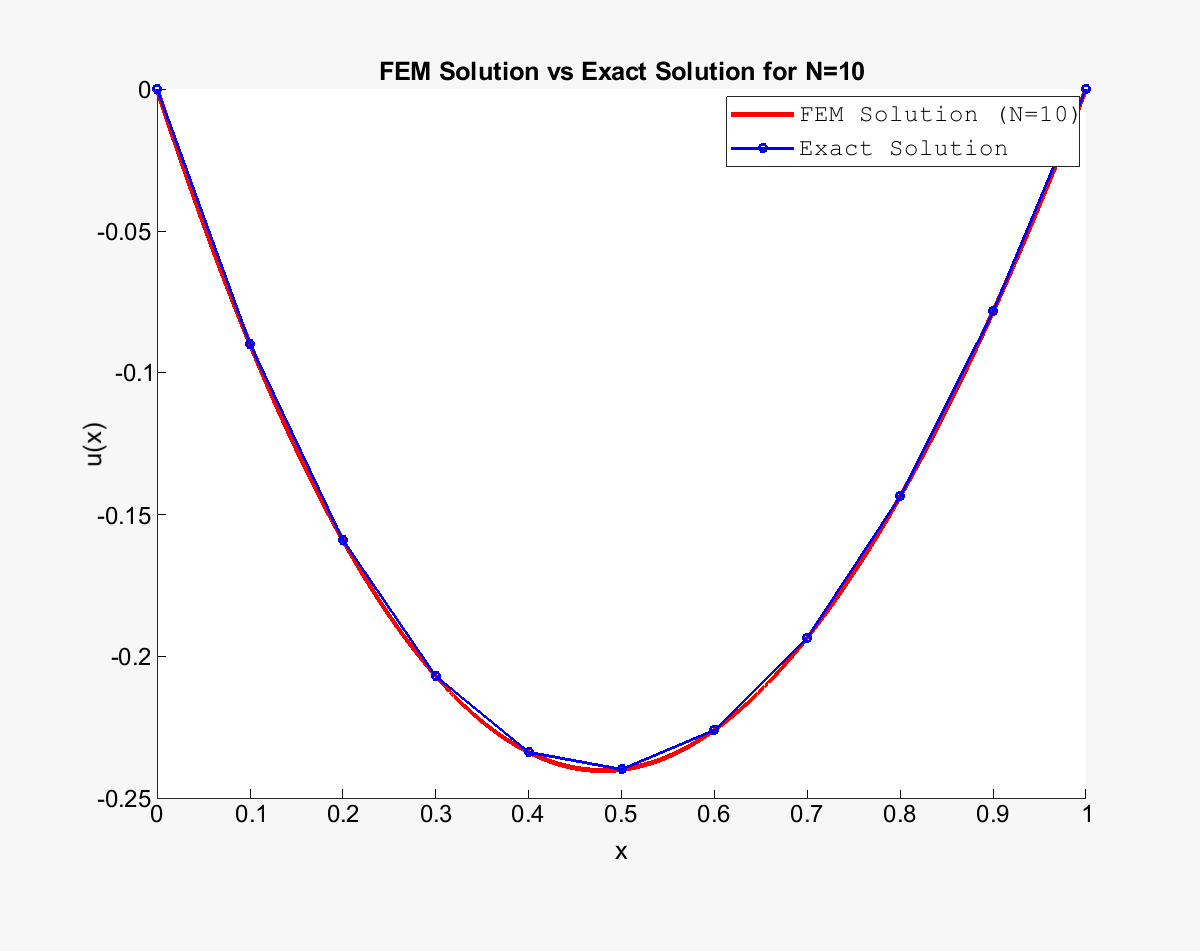
\includegraphics[width=\linewidth]{10.png}
        \caption{$ N=10 $ }
        \label{fig:sub1}
    \end{subfigure}
    \begin{subfigure}{0.4\textwidth}
        \centering
        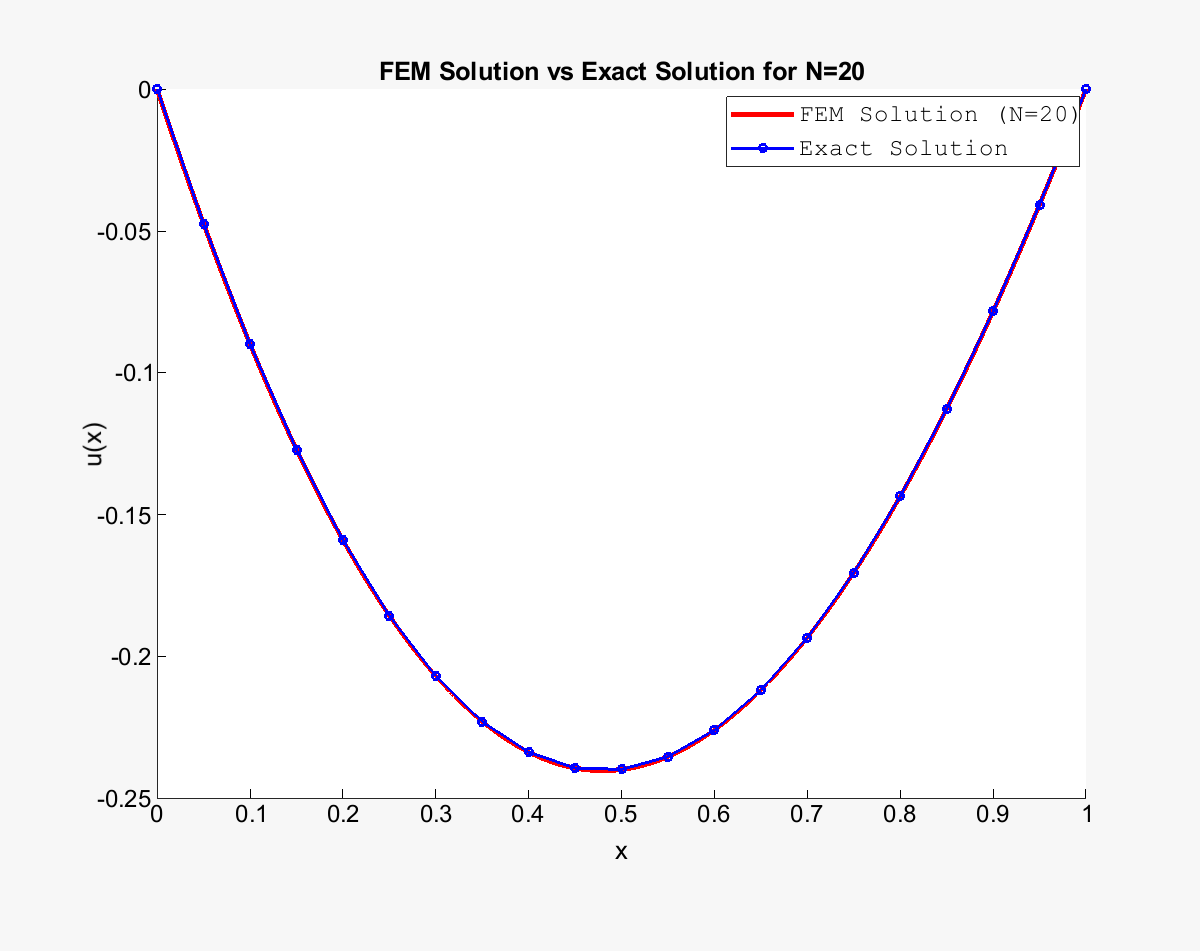
\includegraphics[width=\linewidth]{20.png}
        \caption{$ N=20 $ }
        \label{fig:sub2}
    \end{subfigure}
    
    % 第二行的两张图
    \vspace{0.5em}
    
    \begin{subfigure}{0.4\textwidth}
        \centering
        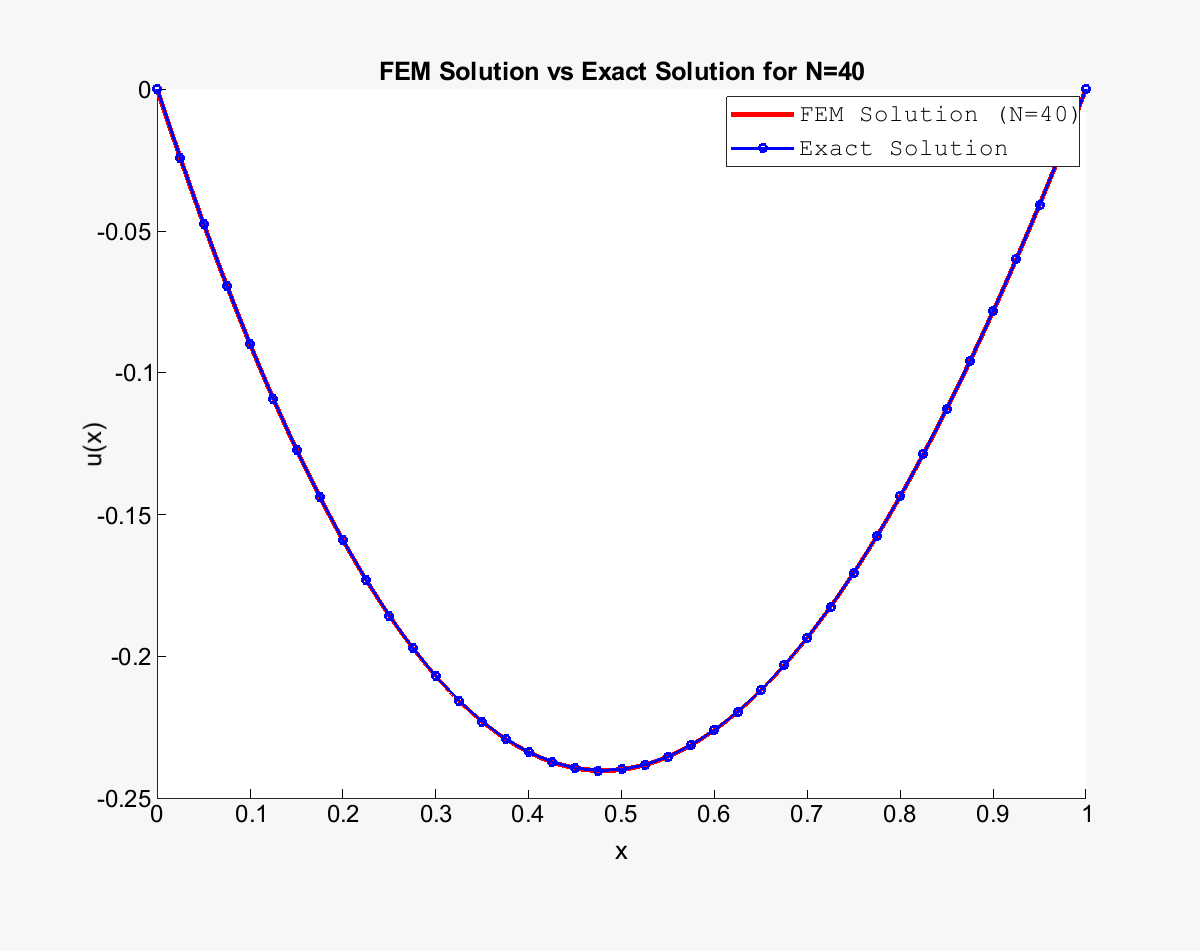
\includegraphics[width=\linewidth]{40.png}
        \caption{$ N=40 $ }
        \label{fig:sub3}
    \end{subfigure}
    \begin{subfigure}{0.4\textwidth}
        \centering
        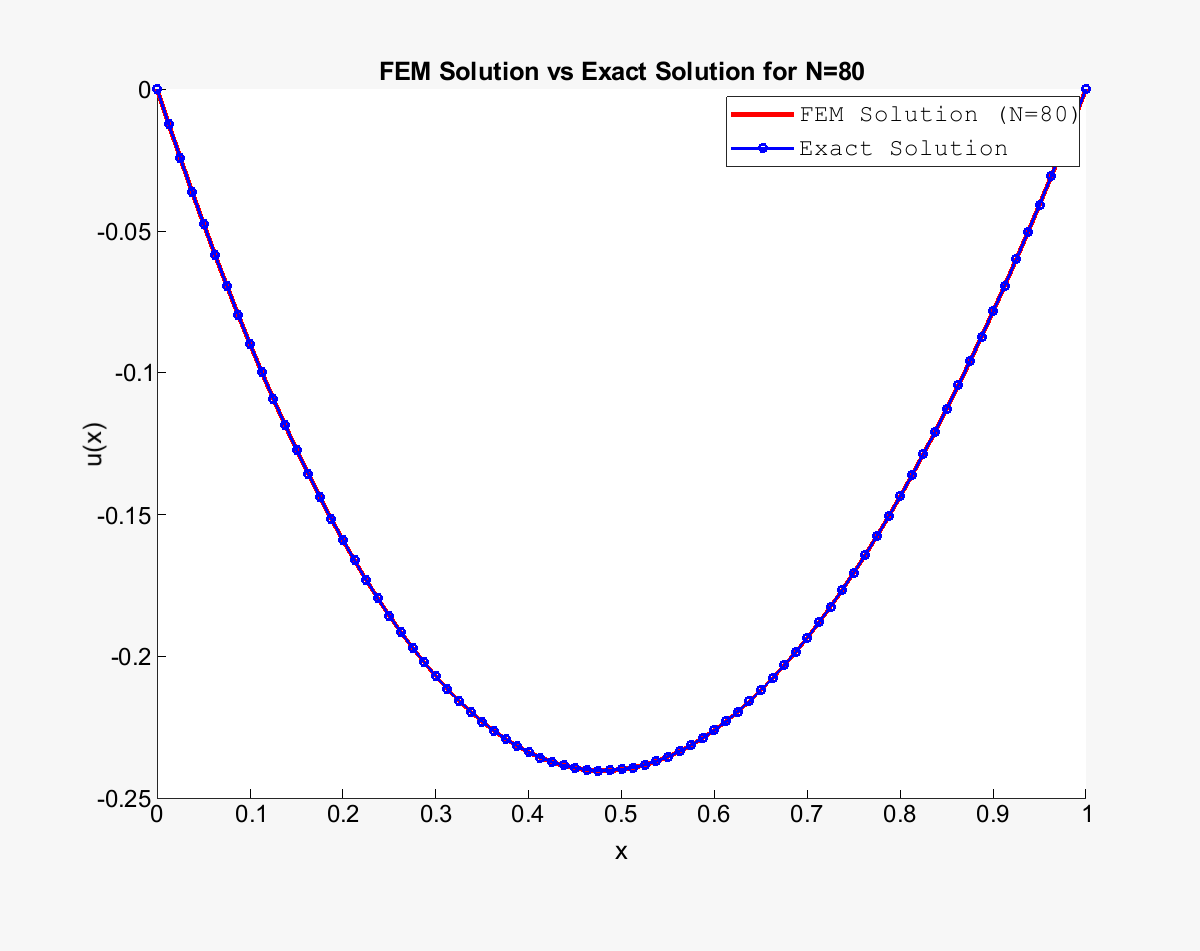
\includegraphics[width=\linewidth]{80.png}
        \caption{$ N=80 $ }
        \label{fig:sub4}
    \end{subfigure}
    
    \caption{北大天元绘制的拟合图像}
    \label{fig:fit}
\end{figure}

\subsection{误差分析}
由于已知其解析解为:
\begin{equation}
    u(x) = (x - 1) \sin x.
\end{equation}
完成数值求解后,使用 $L^2$ 范数和 $H^1$ 范数计算误差,对结果进行讨论。

$L^2$ 范数的定义为:
\begin{equation}
    \| e \|_{L^2} = \left( \int_0^1 (u(x) - u_h(x))^2 \, dx \right)^{1/2},
\end{equation}

$H^1$ 范数的定义为:
\begin{equation}
    \| e \|_{H^1} = \left( \int_0^1 \left( (u(x) - u_h(x))^2 + (u'(x) - u_h'(x))^2 \right) dx \right)^{1/2}.
\end{equation}
其中,实验中利用差分计算导数。

得到如下结果:

% Table generated by Excel2LaTeX from sheet 'Sheet1'
\begin{table}[htbp]
	\centering
	\caption{误差分析}
	  \begin{tabular}{|c|cc|cc|}
	  \toprule
	  N     & \multicolumn{1}{c}{$L^2$ error} & \multicolumn{1}{c|}{order} & \multicolumn{1}{c}{$H^1$ error} & \multicolumn{1}{c|}{order} \\
	  \midrule
	  10    & $1.70\times 10^{-3}$ &   -    & $5.39\times 10^{-2}$ & - \\
	  20    & $4.26\times 10^{-4}$ & 2.00 & $2.69\times 10^{-2}$ & 1.00 \\
	  40    & $1.07\times 10^{-4}$ & 2.00 & $1.34\times 10^{-2}$ & 1.00 \\
	  80    & $2.66\times 10^{-5}$ & 2.00 & $6.68\times 10^{-3}$ & 1.01 \\
	  \bottomrule
	  \end{tabular}%
	\label{tab:error}%
  \end{table}%
  
\section{Discussion}
本节着重进行误差分析,令 $ v\in V_h $ 为一分片线性函数,满足:
\begin{equation}
	v(x_i) = u(x_i)\quad \forall i = 1,2,\cdots,N
\end{equation}
其中 u 是两点边值问题的古典解。

令 e = v - u, 那么考虑区间 $ [a,b] $上的 $ C^1 $函数 $ f $,满足 $ f(a) = f(b) = 0 $,那么 $ |f|<\frac{b-a}{2}\max|f'| $,积分
\begin{equation}
	\int_a^b |f(x)| dx < \frac{b-a}{2}\max|f'|
\end{equation}

结合上式和微分中值定理可得,对于 $ e,e' $有:
\begin{equation}
	\begin{aligned}
		\sup_x|e'| \le C_1h\sup_x|u''|\\
		\sup_x|e| \le C_2h^2\sup_x|u''|
	\end{aligned}
\end{equation}

那么:
\begin{equation}
	\begin{aligned}
		||u-v||_2 \le C_1h^2\sup_x|u''|\\
		||u'-v'||_2 \le C_2h\sup_x|u''|
	\end{aligned}
\end{equation}

因此,$ L^2 $ 误差和 $ H^1 $ 误差的阶数分别为 2 和 1,和实验结果一致。

\appendix
\section{Code}

\begin{lstlisting}[caption={FEM Solver}]
function [x, u_h] = fem_solver(N,F_load)
    % Mesh generation
    a = 0; b = 1;  % Interval [0,1]
    h = (b - a) / N;  % Step size
    x = linspace(a, b, N+1);  % Mesh points
    % Preallocate index and value arrays for the sparse matrix
    I = zeros(3*N-5, 1);  % Row indices
    J = zeros(3*N-5, 1);  % Column indices
    S = zeros(3*N-5, 1);  % Non-zero values
    index = 0;  % Index counter
    % Construct the sparse matrix K

    for i = 1:N-1
        index = index + 1;
		% Diagonal element
        I(index) = i;J(index) = i;S(index) = 2/h; 
        if i > 1
			% Lower diagonal element
            index = index+1;I(index) = i;J(index) = i-1;S(index) = -1/h;  
        end
        if i < N-1
			% Upper diagonal element
            index = index+1;I(index) = i;J(index) = i+1;S(index) = -1/h;  
        end
    end

    % Construct the sparse matrix K using the sparse function
    K = sparse(I, J, S, N-1, N-1);
    % Construct the load vector F
    F = zeros(N-1, 1);
    for j = 1:N-1
        F(j) = F_load(j,h);
    end
    % Solve the linear system K * u_h = F
    u_h = K \ F;
    % Apply boundary conditions u(0) = 0 and u(1) = 0
    u_h = [0, u_h', 0];
end
\end{lstlisting}

\begin{lstlisting}[caption={Main Code}]
% Main script: Call FEM solver and plot results for different N values
Ns = [10, 20, 40, 80];  % Different values for N
u_exact = @(x) (x - 1) .* sin(x);  % Exact solution
u_exact_der = @(x) sin(x)+(x-1).*cos(x);
% Load function integrate f*phi
F_load = @(i,h) 4*(h*i - 1) * sin(h/2)^2 * sin(h*i)/h - 2*sin(h) * cos(h*i); 
				
num = 10000;
delta_x = 1/num;
x = linspace(0,1,num);
u_exact_values = u_exact(x);
L2_error_list = zeros(1,4);
L2_diff_error_list = zeros(1,4);

for i = 1:length(Ns)
    N = Ns(i);   
    % Call FEM solver to get mesh points and FEM solution
    [x_sample, u_sample] = fem_solver(N,F_load);
    % Calculate the exact solution at mesh points
    u_h = interp1(x_sample,u_sample, x);
    % Compute the L2 norm error
    L2_error = sqrt(sum((u_h - u_exact_values).^2)*delta_x);
    u_diff_h = diff(u_h)/delta_x;
    u_diff_exact = diff(u_exact_values)/delta_x;
    L2_diff_error = sum((u_diff_h - u_diff_exact).^2)*delta_x;
    L2_diff_error = sqrt(L2_error^2 + L2_diff_error);    
    % Print the error
	fprintf('L2 norm error with N=%d: %e\n', N, L2_error);
	fprintf('LH1 norm error with N=%d: %e\n', N, L2_diff_error);
	L2_error_list(i) = L2_error;
	L2_diff_error_list(i) = L2_diff_error;
end

for i = 2:length(Ns)
    N_now = Ns(i);
    N_old = Ns(i-1);
    order_l2 = log(L2_error_list(i-1)/L2_error_list(i))/log(N_now/N_old);
    order_l2_diff = log(L2_diff_error_list(i-1)/L2_diff_error_list(i))/log(N_now/N_old);
    fprintf("N:%d, L2 order:%e, LH1 order:%e\n",N_now,order_l2,order_l2_diff);
end
\end{lstlisting}

\end{document}
